
Consider the polyhedron defined by the following constraints:
\begin{align*}
x_1+x_2 &\leq 1,\\
-x_1+2x_2 &\leq 2,\\
x_1,x_2 & \geq 0.
\end{align*}

\begin{center}
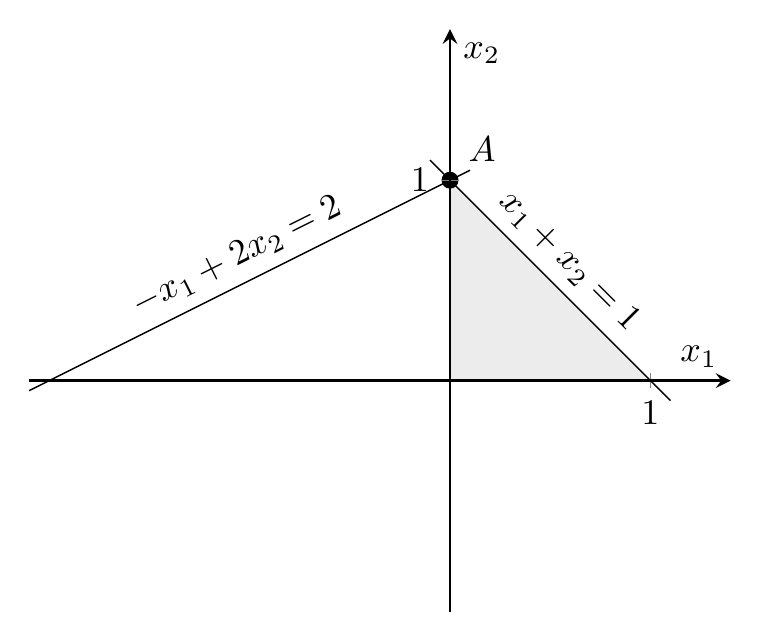
\begin{tikzpicture}[scale=1.3]
\begin{axis}[ xlabel={$x_1$}, ylabel={$x_2$}
    ,axis lines=middle
    ,axis equal
    ,axis on top=true
    ,xtick = {1}
    ,ytick = {1}
,samples=41, thick,
,domain=-0.5:8, xmin=-2.1, xmax=1.4,
    ymin=-0.5, ymax=1.1,
]
\fill[lightgray!30] (0,0) -- (0,1) -- (1,0) -- (0,0) -- cycle;
\addplot+ [mark=none,mark color=black, color=black, thin,domain=-0.1:1.1]{1-x}node[pos=0.5,sloped,above] {$x_1+x_2=1$};
\addplot+ [mark=none,mark color=black, color=black, thin,domain=-2.1:0.1]{1+0.5*x}node[pos=0.5,sloped,above] {$-x_1+2x_2=2$};
\draw (0,5) circle[radius=2.2pt];
\fill (0,5)  circle[radius=2.2pt];
\node [circle,fill=black,draw,scale=0.2,label=above right:$A$] at (0,1) {A};
\end{axis}
\end{tikzpicture}
\end{center}



In standard form, after introducing the two slack variables $x_3$ and
$x_4$,  we have
\begin{align*}
x_1+x_2+x_3 & =1,\\
-x_1+2x_2+x_4 &=2,\\
x_1,x_2,x_3,x_4 & \geq 0.
\end{align*}
The vertex $A$ corresponds to $x_1=0$, $x_2=1$, $x_3=0$, $x_4=0$, and is degenerate. 
Consider the case where the  variables  $x_1$ and $x_2$ are in the basis.
Calculate all basic directions, determine if they are feasible of not, and
represent them on the picture.

